\section{Worksheet 8}
\subsection{Fresnel Reflectance}

\begin{lstlisting}
inline float fresnel_r_s(float cos_theta1, float cos_theta2, float ior1, float ior2)
{
	// Compute the perpendicularly polarized component of the Fresnel reflectance
	return (ior1 * cos_theta1 - ior2 * cos_theta2) / (ior1 * cos_theta1 + ior2 * cos_theta2);
}

inline float fresnel_r_p(float cos_theta1, float cos_theta2, float ior1, float ior2)
{
	// Compute the parallelly polarized component of the Fresnel reflectance
	
	return (ior2 * cos_theta2 - ior1 * cos_theta1) / (ior2 * cos_theta2 + ior1 * cos_theta1);
}

inline float fresnel_R(float cos_theta1, float cos_theta2, float ior1, float ior2)
{
	// Compute the Fresnel reflectance using fresnel_r_s(...) and fresnel_r_p(...)
	float r_s = fresnel_r_s( cos_theta1,  cos_theta2,  ior1,  ior2);
	float r_p= fresnel_r_p(cos_theta1, cos_theta2, ior1, ior2);
	
	return 0.5*(pow(r_s,2)+ pow(r_p, 2));
}
\end{lstlisting}

\begin{lstlisting}
bool RayTracer::trace_refracted(const Ray& in, const HitInfo& in_hit, Ray& out, HitInfo& out_hit, float& R) const
{
	float3 normal;
	float out_ior = get_ior_out(in, in_hit, normal);
	out_hit.ray_ior = out_ior;
	bool refraction = refract(out.direction, in.direction, normal, out_hit.ray_ior / in_hit.ray_ior);
	if (refraction) {
		out.origin = in_hit.position;
		out.tmin = 1e-4;
		out.tmax = RT_DEFAULT_MAX;
		out_hit.trace_depth = in_hit.trace_depth + 1;
		
		float cos_theta1 = dot(in.direction, in_hit.shading_normal);
		float cos_theta2 = dot(out.direction, in_hit.shading_normal);
		R = fresnel_R(cos_theta1, cos_theta2, in_hit.ray_ior, out_hit.ray_ior);
		
		trace_to_closest(out, out_hit);
	}
	else {
		R = 1;
	}
	
	return out_hit.has_hit;
}
\end{lstlisting}

\begin{figure}[H]
	\centering
	\subfloat[\centering R always set to 10\%]{{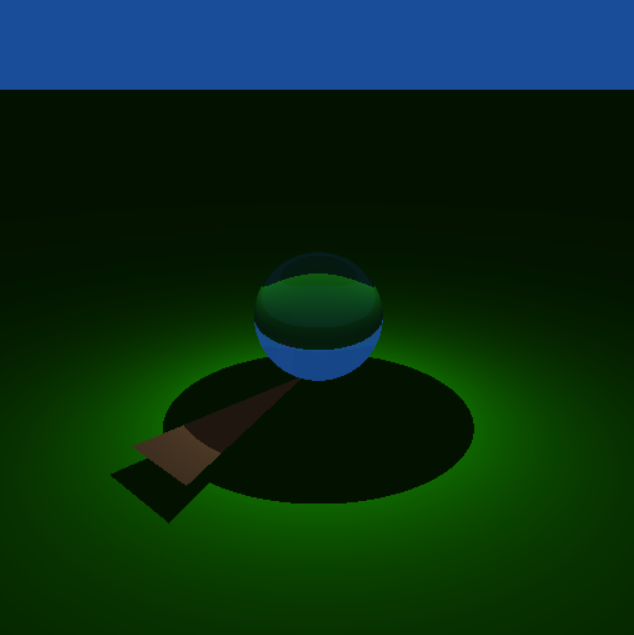
\includegraphics[width=5cm]{images/worksheet_8/10_percent_fresnel} }}%
	\qquad
	\subfloat[\centering Fresnel reflectance]{{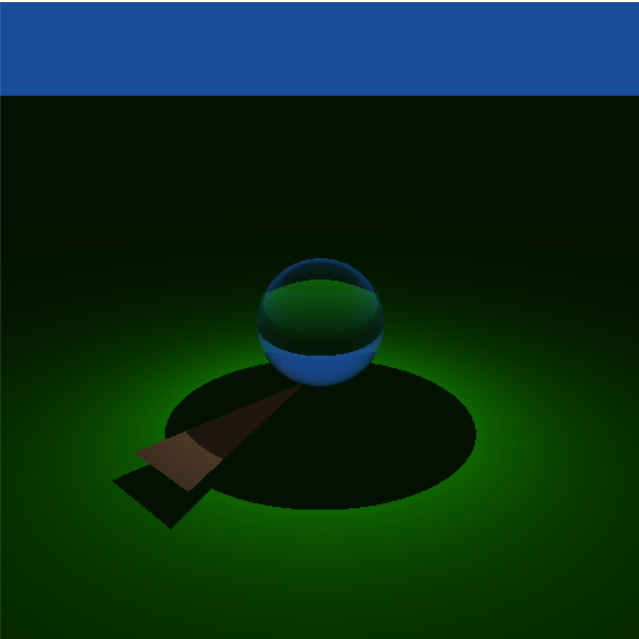
\includegraphics[width=5cm]{images/worksheet_8/fresnel} }}%
	\captionsetup{justification=centering,margin=2cm}
	\caption{Comparison between default 10\% reflectance and fresnel reflectance (Fully transparent material)}%
	%\label{fig:tex_scale_comparison}%
\end{figure}

\begin{figure}[H]
	\centering
	\subfloat[\centering R always set to 10\%]{{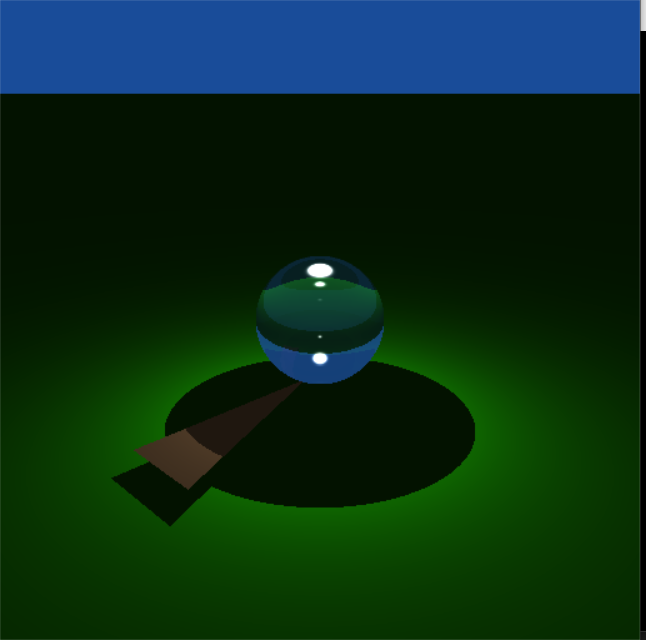
\includegraphics[width=5cm]{images/worksheet_2/part_5} }}%
	\qquad
	\subfloat[\centering Fresnel reflectance]{{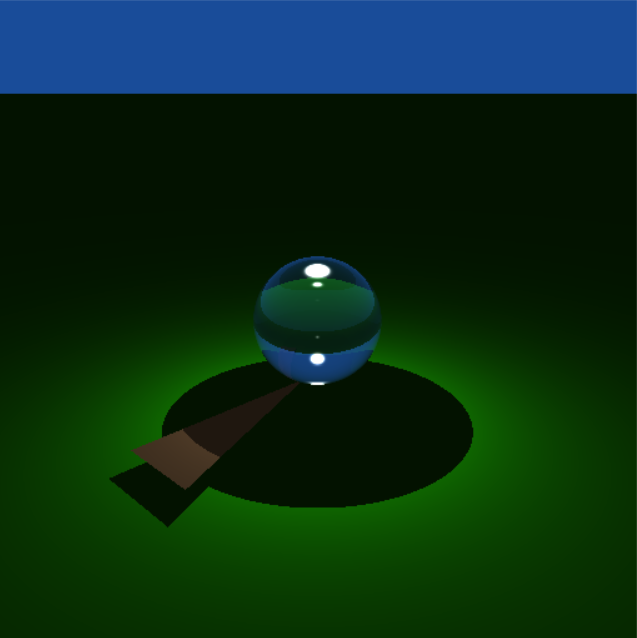
\includegraphics[width=5cm]{images/worksheet_8/default_scene_fresnel} }}%
	\captionsetup{justification=centering,margin=2cm}
	\caption{Comparison between default 10\% reflectance and fresnel reflectance (Glossy material)}%
	%\label{fig:tex_scale_comparison}%
\end{figure}

\begin{figure}[H]
	\centering
	\subfloat[\centering R always set to 10\%]{{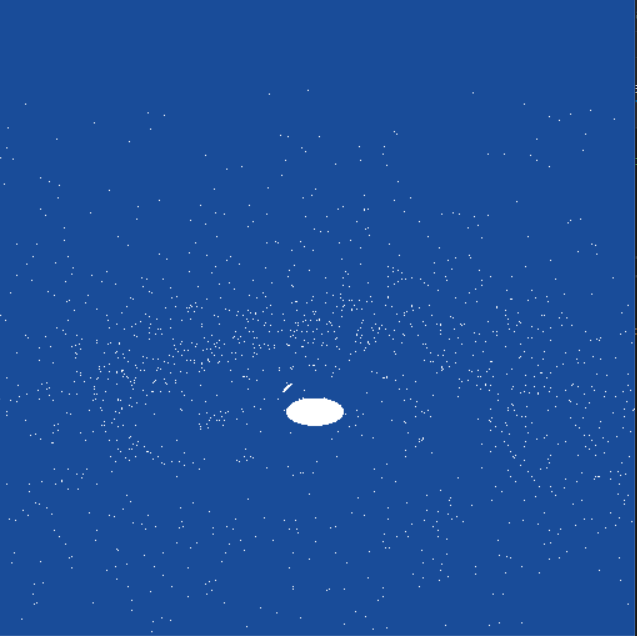
\includegraphics[width=5cm]{images/worksheet_7/caustics_preview} }}%
	\qquad
	\subfloat[\centering Fresnel reflectance]{{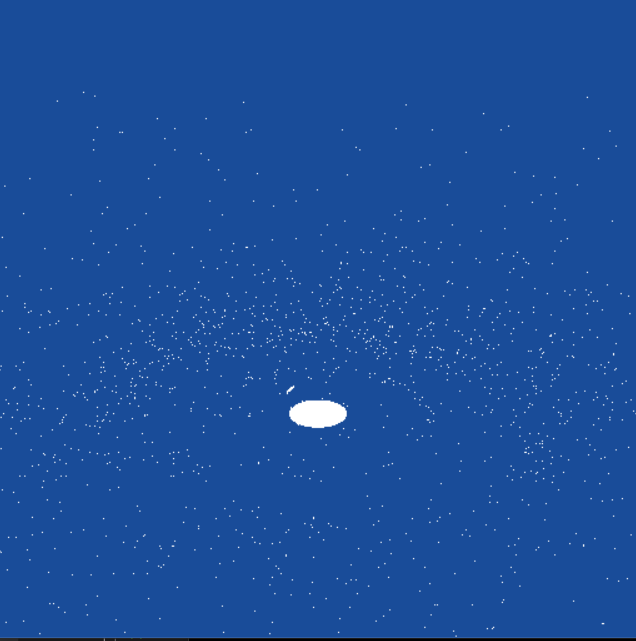
\includegraphics[width=5cm]{images/worksheet_8/caustics_preview_fresnel} }}%
	\captionsetup{justification=centering,margin=2cm}
	\caption{Comparison between default 10\% reflectance and fresnel reflectance(White dots)}%
	%\label{fig:tex_scale_comparison}%
\end{figure}

\begin{figure}[H]
	\centering
	\subfloat[\centering R always set to 10\%]{{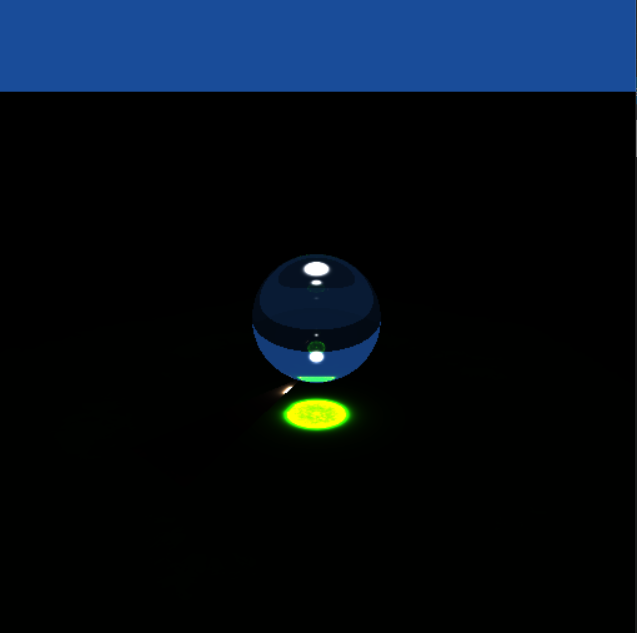
\includegraphics[width=5cm]{images/worksheet_7/caustics_only} }}%
	\qquad
	\subfloat[\centering Fresnel reflectance]{{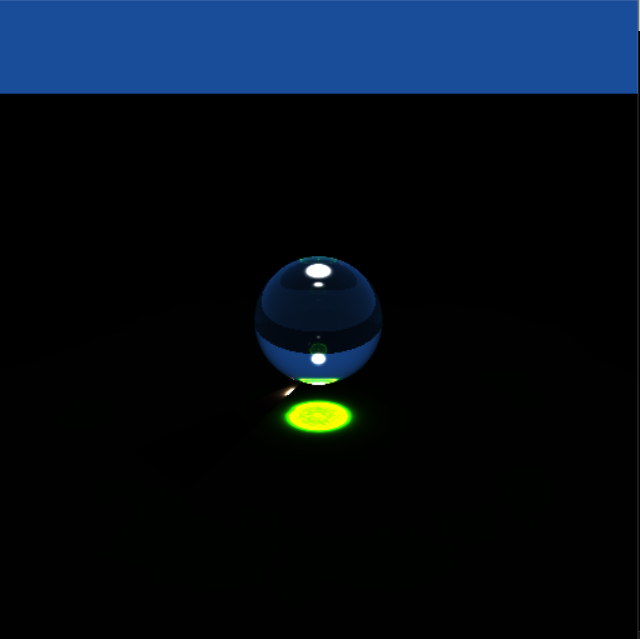
\includegraphics[width=5cm]{images/worksheet_8/caustics_only_fresnel} }}%
	\captionsetup{justification=centering,margin=2cm}
	\caption{Comparison between default 10\% reflectance and fresnel reflectance(Caustics only)}%
	%\label{fig:tex_scale_comparison}%
\end{figure}

\begin{figure}[H]
	\centering
	\subfloat[\centering R always set to 10\%]{{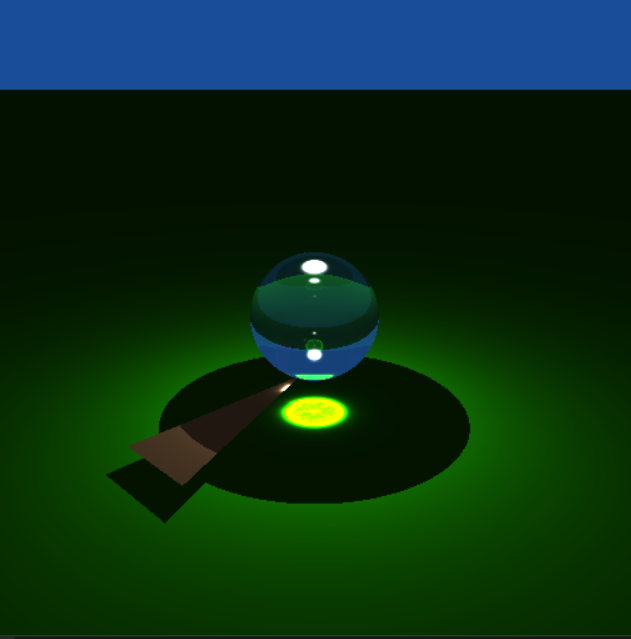
\includegraphics[width=5cm]{images/worksheet_7/caustics_full_illum} }}%
	\qquad
	\subfloat[\centering Fresnel reflectance]{{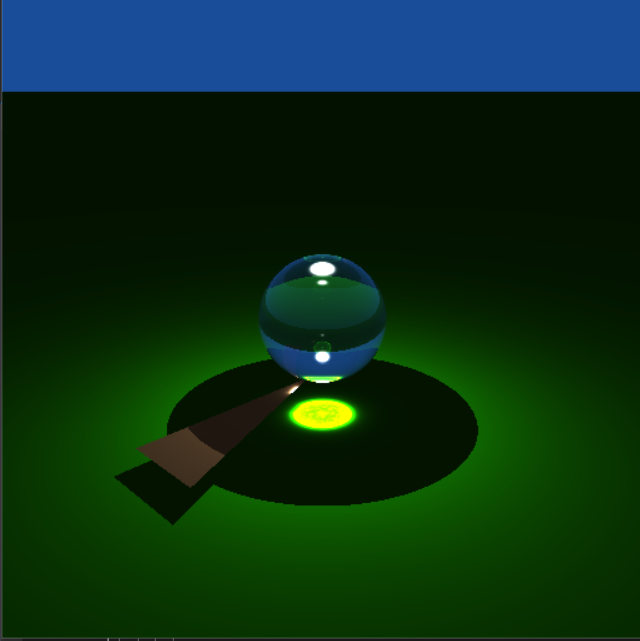
\includegraphics[width=5cm]{images/worksheet_8/caustics_full_illum_fresnel} }}%
	\captionsetup{justification=centering,margin=2cm}
	\caption{Comparison between default 10\% reflectance and fresnel reflectanace(Full illumination)}%
	%\label{fig:tex_scale_comparison}%
\end{figure}

\subsection{Absorbtion}

\begin{lstlisting}
float3 Volume::shade(const Ray& r, HitInfo& hit, bool emit) const
{
	// If inside the volume, Find the direct transmission through the volume by using
	// the transmittance to modify the result from the Transparent shader.
	float3 transmittance = get_transmittance(hit);
	return Transparent::shade(r, hit, emit)*transmittance;
}

float3 Volume::get_transmittance(const HitInfo& hit) const
{
	if(hit.material)
	{
		// Compute and return the transmittance using the diffuse reflectance of the material.
		// Diffuse reflectance rho_d does not make sense for a specular material, so we can use 
		// this material property as an absorption coefficient. Since absorption has an effect
		// opposite that of reflection, using 1/rho_d-1 makes it more intuitive for the user.
		float3 rho_d = make_float3(hit.material->diffuse[0], hit.material->diffuse[1], hit.material->diffuse[2]);
		float3 absorbtion= (1 / rho_d) - 1;
		float3 temp = -absorbtion * hit.dist;
		return make_float3(exp(temp.x), exp(temp.y), exp(temp.z));
	}
	return make_float3(1.0f);
}
\end{lstlisting}

\begin{lstlisting}
float3 GlossyVolume::shade(const Ray& r, HitInfo& hit, bool emit) const
{
	// Compute the specular part of the glossy shader and attenuate it
	// by the transmittance of the material if the ray is inside (as in
	// the volume shader).
	//return 0.9*Transparent::shade(r, hit, emit)+0.1*Mirror::shade(r, hit, emit)+Phong::shade(r, hit, emit);
	
	float3 rho_d = get_diffuse(hit);
	float3 rho_s = get_specular(hit);
	float s = get_shininess(hit);
	
	float3 phong_radiance = make_float3(0.0f);
	
	float3 wo = -r.direction;
	for (int i = 0; i < lights.size(); i++) {
		float3 wi;
		float3 L;
		bool shade = lights[i]->sample(hit.position, wi, L);
		float3 wr = reflect(wi, hit.shading_normal);
		if (dot(wi, hit.shading_normal) > 0) {
			float3 b = rho_s * (s + 2) / (2 * M_PIf);
			float c = pow(dot(wo, wr), s);
			float3 d = b * c;
			float3 e = L * dot(wi, hit.shading_normal);
			phong_radiance = phong_radiance + d * e;
		}
	}
	
	return 0.9 * Transparent::shade(r, hit, emit)+0.1*Mirror::shade(r, hit, emit)+ phong_radiance +Volume::shade(r, hit, emit);
}
\end{lstlisting}

\begin{lstlisting}
float3 ParticleTracer::get_transmittance(const HitInfo& hit) const
{
	if (hit.material)
	{
		// Compute and return the transmittance using the diffuse reflectance of the material.
		// Diffuse reflectance rho_d does not make sense for a specular material, so we can use 
		// this material property as an absorption coefficient. Since absorption has an effect
		// opposite that of reflection, using 1/rho_d-1 makes it more intuitive for the user.
		float3 rho_d = make_float3(hit.material->diffuse[0], hit.material->diffuse[1], hit.material->diffuse[2]);
		float3 absorbtion = (1 / rho_d) - 1;
		float3 temp = -absorbtion * hit.dist;
		return make_float3(exp(temp.x), exp(temp.y), exp(temp.z));
	}
	return make_float3(1.0f);   
}
\end{lstlisting}
Then we edit the case 12 of the switch case of the function ParticleTracer::trace\_particle in the following way.
\begin{lstlisting}
case 12: // absorbing glossy volume
{
	// Handle absorption here (Worksheet 8)
	if(dot(r.direction,hit.geometric_normal)>0)
	Phi = Phi* get_transmittance(hit);
}
\end{lstlisting}
\begin{figure}[H]
	\centering
	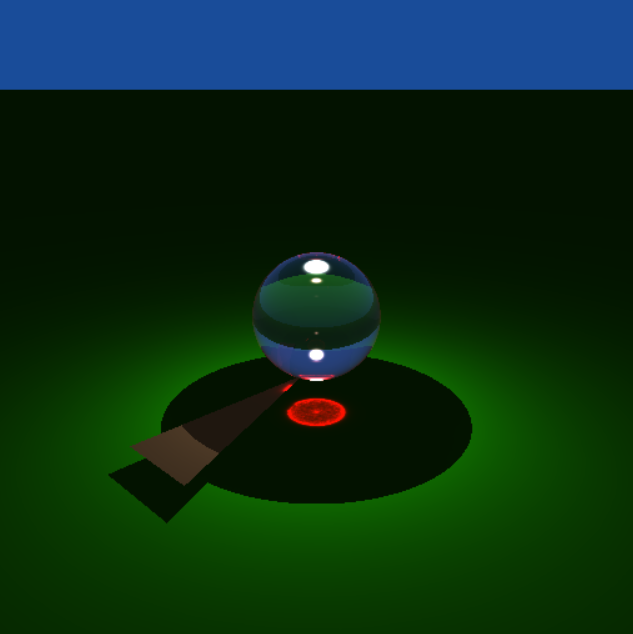
\includegraphics[scale=\imagescale]{images/worksheet_8/final}
	\caption{Final rendering of the default scene}
	\label{fig:final_default}
\end{figure}